\section{Introduction}
\label{sec:intro}

Polyp segmentation networks that are accurate on their training data lose much of that accuracy
at new centres, whose images differ in endoscopes, illumination and
patients~\cite{ali2023polypgen,ali2024endocv}. This gap limits their clinical value: colorectal
cancer is among the leading causes of cancer death~\cite{siegel2024cancer}, and automatic
segmentation aims to help endoscopists, who miss about one in five
polyps~\cite{vanrijn2006miss}. Recent networks reach high Dice on test images from their
training datasets~\cite{fan2020pranet,wei2021sanet,dong2023polyppvt,hu2026pranetv2,sun2026asgnet},
but much lower Dice elsewhere. In our experiments, for example, Polyp-PVT~\cite{dong2023polyppvt}
reaches 93.2\% mean Dice on \mbox{CVC-ClinicDB} but only 78.6\% on ETIS, a dataset from another
hospital. For clinical use, closing this gap matters more than further gains on the training
distribution.

Polyp segmentation also has a symmetry that standard training does not enforce. A mirrored
polyp is still a polyp, so the correct mask of a mirrored image is the mirrored mask. We measure
departures from this flip equivariance with the flip gap: one minus the Dice overlap between the
binary masks predicted for an image and for its flipped copy, once flipped back, averaged over
horizontal and vertical flips. As Fig.~\ref{fig:teaser} shows, the flip gap of trained models
is far from zero, and it is largest on the two hardest test sets, \mbox{CVC-ColonDB} and ETIS.
We hypothesize that a model whose answer changes with a mirror image relies partly on cues that
do not belong to the polyp, and that such cues are unlikely to transfer to new centres.

\begin{figure*}[t]
\centering
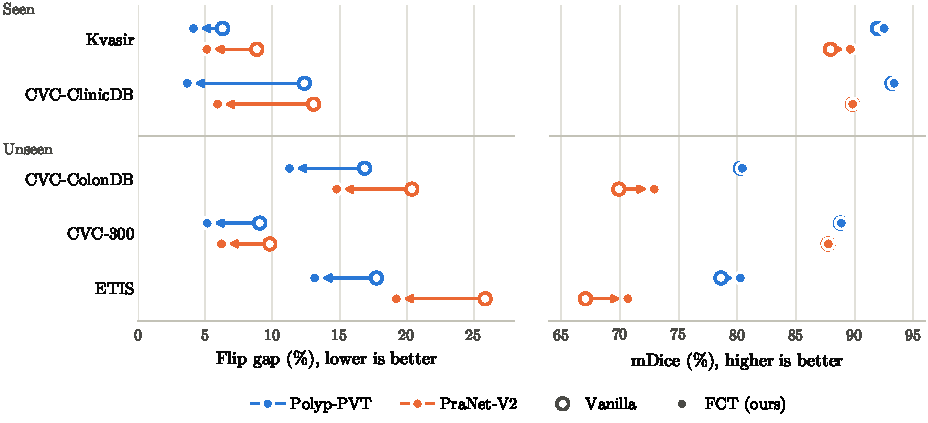
\includegraphics[width=\textwidth]{figures/fig1_flipgap.pdf}
\caption{Flip gap (left; one minus the Dice overlap between the binary masks predicted for an
image and for its flipped copy, once flipped back, averaged over horizontal and vertical flips)
and mDice (right) on five test sets, without (hollow) and with (filled) FCT. Both networks are
least flip-consistent on \mbox{CVC-ColonDB} and ETIS, the two sets where they are least
accurate. FCT lowers the flip gap on every set, and its largest mDice gain, for both networks,
is on ETIS. Means over six seeds.}
\label{fig:teaser}
\end{figure*}

Two remedies are common, and both act on the training loss. Flip augmentation trains on mirrored
copies with mirrored labels, but each copy is constrained only by its own label, never by the
prediction on its mirror. Consistency regularization adds that constraint with a loss term that
penalizes disagreement between the predictions on the views. It comes from semi-supervised
learning, where agreement between views is the only signal that unlabeled images
provide~\cite{laine2017temporal,tarvainen2017mean,sohn2020fixmatch}, and medical variants enforce it
under spatial transformations~\cite{bortsova2019consistency,li2021tcsm}. Since no label says which
view is right, the views are treated as equally reliable or weighed by the model's own confidence.
Supervised uses of consistency, such as AugMix~\cite{hendrycks2020augmix} and
R-Drop~\cite{liang2021rdrop}, keep this symmetry even though the label is known, so a correct view
can be drawn toward a wrong one.

We show that, under full supervision, a consistency term is a reweighted supervised loss. For binary
segmentation, the gradient of a cross-entropy consistency term that draws one view toward the detached
prediction of another equals the supervised gradient, scaled by one minus the ratio of the two views'
errors. Similar decompositions of the distillation gradient are known for
classification~\cite{furlanello2018born,tang2020understanding}; here we apply the identity pixel by
pixel, across views of one image. A consistency term is therefore an adaptive pixel weight on the
supervised loss: positive where a view is farther from the label than its target, and negative where
it is closer. Unweighted consistency mixes both kinds of pixels in every image, and only the label
can tell them apart.

Building on this identity, we propose flip-consistent training (FCT), a plug-in training loss for
polyp segmentation. FCT supervises each image in three orientation views, upright, flipped
horizontally and flipped vertically, and adds a consistency term that draws the predictions of the
views together: each flipped view toward the upright view, and the upright view toward the flipped view
closest to the label. Label-aware weights complete the loss. A flipped view moves toward the upright
view at full strength where it is farther from the label; where it is closer, it moves only if the
upright view is correct, in proportion to how far the upright prediction lies on the correct side of
the 0.5 threshold. This weak term keeps the views consistent without moving either across the
threshold, much as label smoothing tempers overconfident targets~\cite{yuan2020revisiting}, and its
single constant is set by the decision threshold rather than tuned. FCT changes only the training
loss: it multiplies the training time by about 3.5 and adds nothing at inference. To the best of our
knowledge, FCT is the first consistency loss that uses the label to set, pixel by pixel, the
direction in which the views of an image are drawn together.

We add FCT, without retuning, to three segmentation networks of different design:
Polyp-PVT~\cite{dong2023polyppvt}, built on a pyramid vision transformer;
PraNet-V2~\cite{hu2026pranetv2}, a convolutional network with dual-supervised reverse attention;
and ASGNet~\cite{sun2026asgnet}, which guides its features with spectral cues and already trains
with random flips. Each network is trained with and without FCT under six paired random seeds and
tested on five public test sets, three of which are unseen in training. FCT improves ETIS for all
three networks, by +1.65, +3.61 and +1.69 points, and \mbox{CVC-ColonDB} for PraNet-V2, by +3.01
points, all with paired 95\% confidence intervals above zero. It raises the five-set mean Dice on
every seed for Polyp-PVT and PraNet-V2, and on five of six for ASGNet, whose gain is borderline. FCT
also lowers the five-set mean flip gap of Polyp-PVT and PraNet-V2 by 40\% and 34\%, respectively. On
six more centres from the PolypGen benchmark~\cite{ali2023polypgen}, a label-aware variant improves
the pooled Dice on every seed \pend{(FCT itself is pending)}. A study of the loss terms on Polyp-PVT
shows that the multi-view supervision accounts for most of the gain on ETIS, and that the consistency
term and its weights complete it: FCT is the only variant that improves all five test sets on
average \pend{(one row of the study is still running)}.

Our contributions are summarized as follows:
\begin{itemize}
\item We propose FCT, a plug-in training loss that supervises three orientation views of each image
and draws their predictions together with a label-weighted consistency term. It changes no
architecture and adds no cost at inference.
\item We show that, for binary labels, a consistency term between two views acts pixel by pixel as
the supervised loss with an adaptive weight, which is negative where a view is drawn toward a less
accurate one, and we derive label-aware weights whose single constant is set by the decision
threshold.
\item We evaluate FCT on three architectures, five test sets and six paired seeds with confidence
intervals, and dissect the loss into its terms. It improves ETIS for all three networks, raises the
five-set mean Dice on every seed for two of them, and makes the predictions of both markedly more
flip-consistent.
\end{itemize}
